\documentclass{article}
\usepackage[utf8]{inputenc}
\usepackage[a4paper, total={6.5in, 9.5in}]{geometry}
\usepackage{float}
\usepackage{amsmath}
\usepackage{amssymb}
\usepackage{mathtools}
\usepackage{tensor}
\newcommand{\torseur}[7]{
\tensor[_{#1}]{\left\{ \begin{array}{cc}
  #2 & #5 \
  #3 & #6 \
  #4 & #7
\end{array} \right\}}{_{(\vec{x};\vec{y};\vec{z})}}
}
\usepackage{siunitx}
\sisetup{output-decimal-marker={,},group-minimum-digits=4,abbreviations}
\sisetup{inter-unit-product=\ensuremath{{}\cdot{}}}
\newcommand{\deftable}[2]{%
%\hline
\textbf{B.A.M.E}
\begin{table}[h]
  \centering
  \begin{tabular}{llp{130mm}}%
    %& unité/type & Explication \ \hline
    #1
  \end{tabular}
  \label{tab:#2_units}
\end{table}%
}
\newcommand{\deftablevar}[3]{%
  $#1$ & $\si{#2}$ & #3 \
}
\newcommand{\deftableobj}[3]{%
  $#1$ & \textit{#2} & #3 \
}
\newcommand{\bame}[1]{%
%\hline
\begin{table}[h]
  \centering
  \begin{tabular}{llllp{130mm}}%
    Nom & Vecteur & Direction & Sens & Norme \hline
    #1
  \end{tabular}
\end{table}%
}
\newcommand{\vect}[1]{\overrightarrow{#1}}

\title{Tapis de course}
\author{Ewen Le Bihan}
\date{2020-03-27}

\begin{document}

\maketitle

\section{}

\subsection{}

\begin{table}[h]
  \centering
  \begin{tabular}{ll}
    FT1.111 & Moteur AC \\
    FT1.112 & \\
    FT1.113 &
  \end{tabular}
\end{table}

\subsection{}

\begin{equation*}
  \begin{split}
    P_{19} &= C_{u19} \cdot N_{19} \cdot \frac{2\pi}{60} \\
           &= 3.8 \cdot 3400 \cdot \frac{2\pi}{60} \\
           &= \SI{1350}{\watt}
  \end{split}
\end{equation*}

\subsection{}

$P_n > P_{19}$ et $N_{\text{max}} > N_{19}$ donc le choix est adapté

\subsection{}

\begin{equation*}
  \begin{split}
    E &= k_E \cdot \omega \\
    &= 0.33 \cdot 3400 \cdot \frac{2\pi}{60} \\
    &= \SI{117.5}{\volt}
  \end{split}
\end{equation*}

\subsection{}

\begin{equation*}
  \begin{split}
    U &= E + RI \\
      &= E + R\frac{C}{K_T} \\
      &= 117.5 + 1.1\frac{3.8}{0.33} \\
      &= \SI{130}{\volt}
  \end{split}
\end{equation*}

\subsection{}

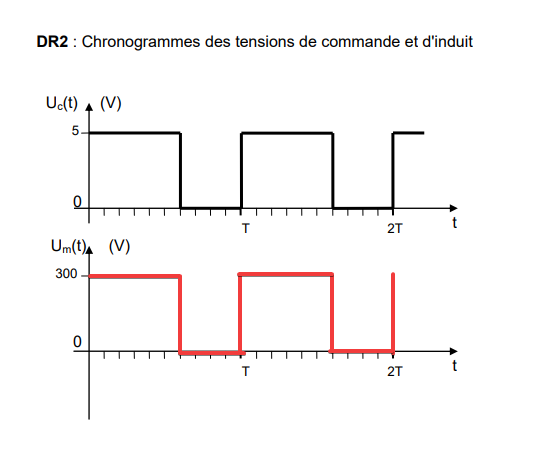
\includegraphics{dr2.png}

\subsection{}

\begin{equation*}
  \begin{split}
    \alpha &= \frac{U_n}{U_G} \\
           &= \frac{130}{300} \\
           &= 0.43
  \end{split}
\end{equation*}

\subsection{}

$\alpha \in [0; 1]$, donc $\alpha$ est admissible.

\end{document}
